% !TeX root = construct.tex

\selectlanguage{hebrew}

\chapter{אני מסתפק בסרגל )ועוד משהו(}

%%%%%%%%%%%%%%%%%%%%%%%%%%%%%%%%%%%%%%%%%%%%%%%%%%%%%%%%%%%%%%%


האם כל בנייה בסרגל ומחוגה ניתנת לבנייה עם סרגל בלבד? התשובה היא שלילית. ב-%
$1822$
המתיטיקאי הצרפתי
\L{Jean-Victor Poncelet}
שיער שכן ניתן להסתפק בסרגל בלבד, בתנאי שקיים במישור מעגל
\textbf{%
אחד%
}.
המשפט הוכח ב-
$1833$
על ידי המתימטיקאי השוויצרי
\L{Jakob Steiner}.
בפרק זה אביא את הוכחת המשפט המבוססת על ההוכחה שמופיעה כבעייה
$34$
ב-%
\L{\cite{dorrie1}},
ועובדה על ידי
\L{Michael Woltermann} \L{\cite{dorrie2}}.%
\footnote{%
ברצוני להודות לו על הרשות להתשמש בעבודתו.
}

%%%%%%%%%%%%%%%%%%%%%%%%%%%%%%%%%%%%%%%%%%%%%%%%%%%%%%%%%%%%%%%


כל צעד בבנייה על סרגל ומחוגה הוא אחת משלושת פעולות האלו:
\begin{itemize}
\setlength{\itemsep}{0pt}
\item
מציאת נקודת החיתוך של שני קווים ישרים.
\item
מציאת נקודות החיתוך של קו ישר עם מעגל.
\item
מציאת נקודות החיתוך של שני מעגלים.
\end{itemize}
ברור שניתן לבצע את הפעולה הראשונה עם סרגל בלבד. עלינו להראות שעבור שתי הפעולות האחרות ניתן למוצא בנייה שקולה המשתמשת רק בסרגל עם מעגל אחד.

%%%%%%%%%%%%%%%%%%%%%%%%%%%%%%%%%%%%%%%%%%%%%%%%%%%%%%%%%%%%%%%

מה המשמעות של בנייה עם סרגל בלבד? מעגל מוגדר על ידי נקודה
$O$,
שהיא מרכז המעגל, וקטע קו באורך
$r$,
הרדיוס, שאחת מהנקודות הקצה שלה היא
$O$.
אם נצליח לבנות את הנקודות
$X,Y$
המסומנות בהתרשים שלהלן, נוכל לטעון שהצלחנו לבנות את נקודות החיתוך של מעגל נתון עם קו נתון ושל שני מעגלים נתונים. המעגלים המצויירים בקו מקווקוו לא ממש מפיעים בבנייה. בהמשך, המעגל היחיד הנתון יצוייר בקו רגיל, ומעגלים המשמשים רק להדגמת הבנייה והוכחתה יהיו מקווקווים.


\begin{center}
\selectlanguage{english}
\begin{tikzpicture}[scale=.9]
\fill (0,0) node[above right] {$O$} circle[radius=1.5pt];
\draw[thick,dashed,name path=circle] (0,0) circle[radius=2cm];
\draw (0,0) -- node[left] {$r$} ++(-60:2cm);
\fill (0,0) ++(-60:2cm) circle[radius=1.5pt];
\draw[name path=line] (-3,-.5) -- ++(20:6cm);
\path [name intersections={of=circle and line,by={X,Y}}];
\fill (X) node[above right,xshift=-2pt,yshift=4pt] {$X$} circle[radius=1.5pt];
\fill (Y) node[above left] {$Y$} circle[radius=1.5pt];
\begin{scope}[xshift=6cm]
\fill (0,0) node[above right] {$O_1$} circle[radius=1.5pt];
\fill (3,0) node[above right] {$O_2$} circle[radius=1.5pt];
\draw[thick,dashed,name path=circle1] (0,0) circle[radius=2cm];
\draw[thick,dashed,name path=circle2] (3,0) circle[radius=2cm];
\draw (0,0) -- node[left] {$r_1$} ++(-70:2cm);
\draw (3,0) -- node[left,below] {$r_2$} ++(-20:2cm);
\fill (0,0) ++(-70:2cm) circle[radius=1.5pt];
\fill (3,0) ++(-20:2cm) circle[radius=1.5pt];
\path [name intersections={of=circle1 and circle2,by={X,Y}}];
\fill (X) node[above,yshift=4pt] {$X$} circle[radius=1.5pt];
\fill (Y) node[below,yshift=-4pt] {$Y$} circle[radius=1.5pt];
\end{scope}
\end{tikzpicture}
\selectlanguage{hebrew}
\end{center}


%%%%%%%%%%%%%%%%%%%%%%%%%%%%%%%%%%%%%%%%%%%%%%%%%%%%%%%%%%%%%%%


תחילה נביא חמש בניות עזר נחוצות )סעיפים
\L{\ref{s.parallel}--\ref{s.root}}%
(,
ואחר כך נראה איך למצוא נקודות חיתוך של קו עם מעגל )סעיף
\L{\ref{s.line-circle-straight}}%
( ושל שני מעלגים )סעיף
\L{\ref{s.circle-circle}}%
(.


%%%%%%%%%%%%%%%%%%%%%%%%%%%%%%%%%%%%%%%%%%%%%%%%%%%%%%%%%%%%%%%

\section{%
בניית קו המקביל לקו נתון%
}\label{s.parallel}

\textbf{%
נתון קו
$l$
המוגדר על ידי שתי נקודות
$A,B$,
ונקודה 
$P$
)שאיננה על הקו(, ניתן לבנות קו דרך
$P$
המקביל ל-%
$AB$.%
}

נפריד את הבנייה לשני מקרים:

\np

\begin{itemize}
\item
"קו מכוון": נתונה הנקודה 
$M$
\textbf{%
החוצה
}
את
$AB$.
\item
כל קו אחר.
\end{itemize}

\vspace{-2ex}

\textbf{%
מקרה ראשון, קו מכוון:
}
נבנה קרן הממשיכה את
$AP$,
ונבחר
$S$,
נקודה כלשהי על הקרן מעבר ל-%
$P$.
נבנה את הקווים
$SB$, $SM$, $BP$.
נסמן ב-%
$O$
את נקודת החיתוך של 
$BP$
עם
$SM$.
נבנה קרן הממשיכה את
$AO$
ונסמן ב-%
$Q$
את החיתוך של הקרן
$AO$
עם
$SB$.
\begin{center}
\selectlanguage{english}
\vspace*{-4pt}
\begin{tikzpicture}
\draw[name path=pq] (-4,0) -- (4,0);
\draw (-2,-2) node[below left] {$A$} coordinate (A) -- (2,-2) node[below right] {$B$} coordinate (B);
\fill (A) circle[radius=1.5pt];
\fill (B) circle[radius=1.5pt];
\draw[name path=as] (A) -- ++(50:4cm) node[above] {$S$} coordinate (S);
\fill (S) circle[radius=1.5pt];
\draw[name path=sb] (S) -- (B);
\path [name intersections={of=pq and as,by={P}}];
\path [name intersections={of=pq and sb,by={Q}}];
\fill (P) node[above left] {$P$} circle[radius=1.5pt];
\fill (Q) node[above right] {$Q$} circle[radius=1.5pt];
\draw[name path=pb] (P) -- (B);
\draw[name path=qa] (Q) -- (A);
\path [name intersections={of=pb and qa,by={O}}];
\fill (O) node[right,xshift=2pt] {$O$} circle[radius=1.5pt];
\fill (0,-2) coordinate (M) node[below right] {$M$} circle[radius=1.5pt];
\draw (S) -- (M);
\end{tikzpicture}
\vspace*{-4pt}
\selectlanguage{hebrew}
\end{center}

\textbf{%
טענה:
$PQ$
מקביל ל-%
$AB$.}

\textbf{הוכחה:}
נשתמש במשפט של
\L{Ceva}
שנוכיח בהמשך.

\textbf{משפט \L{(Ceva)}:}
נתונים שלושה קטעי קו מקודקודי משולש לצלעות הנגדיים שנפגשים בנקודה )כמו בתרשים, אבל 
$M$
לא בהכרח חוצה הצלע(, קטעי הצלעות מקיימים את היחס:
\[
\frac{AM}{MB}\cdot\frac{BQ}{QS}\cdot\frac{SP}{PA} = 1\,.
\]
בבנייה למעלה, 
$M$
חוצה את
$AB$
ולכן
$\disfrac{AM}{MB}=1$.
הגורם הראשון של המכלפה מצטמצם ונקבל את המשוואה:
\selectlanguage{english}
\begin{equation}
\frac{BQ}{QS}=\frac{PA}{SP}=\frac{AP}{PS}\,.\label{eq.ceva}
\end{equation}
\selectlanguage{hebrew}

\vspace{-3ex}

נוכיח ש-%
$\triangle ABS\sim\triangle PQS$,
ולכן הקו
$PQ$
מקביל לקו
$AB$
כי
$\angle ABS = \angle PQS$.
ההוכחה שהמשולשים דומים היא:
\vspace*{-10pt}
\erh{14pt}
\selectlanguage{english}
\begin{equationarray*}{rcl}
BS&=&BQ+QS\\
\disfrac{BS}{QS}&=&\disfrac{BQ}{QS}+\disfrac{QS}{QS} = \disfrac{BQ}{QS}+1\\
AS&=&AP+PS\\
\disfrac{AS}{PS} &=& \disfrac{AP}{PS} + \disfrac{PS}{PS} = \disfrac{AP}{PS} + 1\\
%\end{equationarray*}
%\erh{12pt}
%\selectlanguage{english}
%\begin{equationarray*}{rcl}
\disfrac{BS}{QS}=\disfrac{BQ}{QS}+1&=&\disfrac{AP}{PS} + 1=\disfrac{AS}{PS}\,,
\end{equationarray*}
\selectlanguage{hebrew}
כאשר המשוואה האחרונה מתקבלת מהמשוואה
\L{\ref{eq.ceva}}.

\np

\textbf{הוכחה של משפט \L{Ceva}:}
נתבונן בתרשימים שלהן:
\begin{center}
\selectlanguage{english}
\vspace*{-4pt}
\begin{tikzpicture}
\path[name path=pq] (-4,0) -- (4,0);
\draw (-2,-2) node[below left] {$A$} coordinate (A) -- (2,-2) node[below right] {$B$} coordinate (B);
\coordinate (M) at (0,-2);
\draw[name path=as] (A) -- ++(50:4cm) node[above] {$S$} coordinate (S);
\draw[name path=sb] (S) -- (B);
\path [name intersections={of=pq and as,by={P}}];
\path [name intersections={of=pq and sb,by={Q}}];
\path[name path=pb] (P) -- (B);
\path[name path=qa] (Q) -- (A);
\path [name intersections={of=pb and qa,by={O}}];
\draw[fill=gray!40] (B) -- (O) -- (Q);
\draw[fill=gray!70] (S) -- (O) -- (Q);
\draw (B) -- (O) -- (A);
\draw (S) -- (O) -- (A);
\draw (A) -- (B) -- (S) -- cycle;
\draw (S) -- (O);
\draw (B) -- (O);
\fill (A) circle[radius=1.5pt];
\fill (B) circle[radius=1.5pt];
\fill (S) circle[radius=1.5pt];
\fill (Q) node[above right] {$Q$} circle[radius=1.5pt];
\fill (O) node[above left] {$O$} circle[radius=1.5pt];
\path[name path=al1] (O) -- ($(Q)!(O)!(B)$);
\draw[rotate=-155] ($(Q)!(O)!(B)$) rectangle +(7pt,7pt);
\path [name intersections={of=al1 and sb,by={A1}}];
\draw[thick,dashed] (O) -- (A1);
\begin{scope}[xshift=6cm]
\path[name path=pq] (-4,0) -- (4,0);
\draw (-2,-2) node[below left] {$A$} coordinate (A) -- (2,-2) node[below right] {$B$} coordinate (B);
\coordinate (M) at (0,-2);
\draw[name path=as] (A) -- ++(50:4cm) node[above] {$S$} coordinate (S);
\draw[name path=sb] (S) -- (B);
\path [name intersections={of=pq and as,by={P}}];
\path [name intersections={of=pq and sb,by={Q}}];
\draw[name path=pb] (P) -- (B);
\draw[name path=qa] (Q) -- (A);
\path [name intersections={of=pb and qa,by={O}}];
\draw (B) -- (O) -- (Q);
\draw (A) -- (Q) -- (B);
\draw[fill=gray!40] (B) -- (Q) -- (A);
\draw[fill=gray!70] (S) -- (Q) -- (A);
\draw (A) -- (B) -- (S) -- cycle;
\draw (S) -- (O);
\draw (B) -- (O);
\fill (A) circle[radius=1.5pt];
\fill (B) circle[radius=1.5pt];
\fill (S) circle[radius=1.5pt];
\fill (Q) node[above right] {$Q$} circle[radius=1.5pt];
\fill (O) node[above left] {$O$} circle[radius=1.5pt];
\path[name path=al2] (A) -- ($(Q)!(A)!(B)$);
\draw[rotate=-155] ($(Q)!(A)!(B)$) rectangle +(7pt,7pt);
\path [name intersections={of=al2 and sb,by={A2}}];
\draw[thick,dashed] (A) -- (A2);
\end{scope}
\end{tikzpicture}
\vspace*{-6pt}
\selectlanguage{hebrew}
\end{center}
אם הגבהים של שני משולשים שוואים, יחס השטחים שווה ליחס הבסיסים.
%\[
%A_1 = \frac{1}{2}hb_1,\quad A_2 = \frac{1}{2}hb_2, \quad \frac{A_1}{A_2}=\frac{b_1}{b_2}\,.
%\]
בכל אחד מהתרשימים, הגבהים של זוג המשולשים המסומנים באפור שווים. לכן:%
\footnote{%
נשתמש בשם המשולש כקיצור לשטחו.%
}
\[
\frac{\triangle BQO}{\triangle SQO} = \frac{BQ}{QS}\;,\quad\quad \frac{\triangle BQA}{\triangle SQA} = \frac{BQ}{QS}\;.
\]
על ידי חיסור של המשולשים המסומנים, נקבל יחס בין המשולשים המסומנים באפור:
\begin{center}
\selectlanguage{english}
\vspace*{-4pt}
\begin{tikzpicture}
\path[name path=pq] (-4,0) -- (4,0);
\draw (-2,-2) node[below left] {$A$} coordinate (A) -- (2,-2) node[below right] {$B$} coordinate (B);
\coordinate (M) at (0,-2);
\draw[name path=as] (A) -- ++(50:4cm) node[above] {$S$} coordinate (S);
\draw[name path=sb] (S) -- (B);
\path [name intersections={of=pq and as,by={P}}];
\path [name intersections={of=pq and sb,by={Q}}];
\path[name path=pb] (P) -- (B);
\draw[thick,name path=qa] (Q) -- (A);
\path [name intersections={of=pb and qa,by={O}}];
\draw[fill=gray!50] (B) -- (O) -- (A);
\draw[fill=gray!70] (S) -- (O) -- (A);
\draw (B) -- (O) -- (A);
\draw (S) -- (O) -- (A);
\draw (A) -- (B) -- (S) -- cycle;
\draw (S) -- (O);
\draw (B) -- (O);
\fill (A) circle[radius=1.5pt];
\fill (B) circle[radius=1.5pt];
\fill (S) circle[radius=1.5pt];
\fill (Q) node[above right] {$Q$} circle[radius=1.5pt];
\fill (O) node[right,xshift=2pt] {$O$} circle[radius=1.5pt];
\end{tikzpicture}
\vspace*{-4pt}
\selectlanguage{hebrew}
\end{center}
\[
\frac{BQ}{QS} = \frac{\triangle BQA - \triangle BQO}{\triangle SQA-\triangle SQO} = \frac{\triangle BOA}{\triangle SOA}\,.
\]
החישוב עלול להיראות חשוד. נסביר אותו תוך שימוש בסימונים פשוטים יותר:
\erh{10pt}
\begin{equationarray*}{rcl}
 \disfrac{c}{d} &=&\disfrac{a}{b}\\
 \disfrac{e}{f} &=&\disfrac{a}{b}\\
c-e &=& \disfrac{ad}{b} - \disfrac{af}{b}= \disfrac{a}{b}(d-f)\\
\disfrac{c-e}{d-f} &=& \disfrac{a}{b}\,.
\end{equationarray*}

\vspace{-2ex}


באופן דומה ניתן להוכיח:
\[
\frac{AM}{MB} = \frac{\triangle AOS}{\triangle BOS}\;,\quad\quad \frac{SP}{PA} =\frac{\triangle SOB}{\triangle AOB}\;,
\]

\np

ומכאן:
\[
\frac{AM}{MB}\cdot\frac{BQ}{QS}\cdot\frac{SP}{PA} = \frac{\triangle AOS}{\triangle BOS}\frac{\triangle BOA}{\triangle SOA}\frac{\triangle SOB}{\triangle AOB}=1\,,
\]

כי סדר הקודקודים במשולש לא משנה:
\[
\triangle AOS=\triangle SOA,\, \triangle BOA=\triangle AOB,\, \triangle SOB=\triangle BOS\,.
\]

\vspace{-4ex}

\textbf{סוף הוכחה של משפט \L{Ceva}}.
%%%%%%%%%%%%%%%%%%%%%%%%%%%%%%%%%%%%%%%%%%%%%%%%%%%%%%%%%%%%%%%

\medskip

\textbf{%
מקרה שני, כל קו אחר:
}
נסמן את הקו ב-%
$l$,
נסמן ב-%
$c$
את
\textbf{%
המעגל הקבוע%
}
שמרכזו בנקודה
$O$
והרדיוס שלו הוא
$r$,
ונסמן ב-%
$P$
את הנקודה שלא נמצאת על הקו שיש לבנות דרכו קו המקביל ל-%
$l$.
עליך להשתכנע שהבנייה לא תלוייה במיקום המעגל במישור או ברדיוס שלו.

נבחר 
$M$,
נקודה כלשהי על הקו 
$l$,
ונבנה קרן הממשיכה את
$MO$
והחותך את המעגל ב-%
$U,V$.
\begin{center}
\selectlanguage{english}
\begin{tikzpicture}[scale=.8]
\coordinate (O) at (0,0);
\fill (O) node[below right] {$O$} circle[radius=1.5pt];
\draw[name path=circle] (O) circle[radius=2cm];
\draw[name path=l] (-4,-3) -- node[above, near end] {$l$} +(9,0);
\path[name path=mo] (-2,-3) coordinate (M) -- ($(-2,-3)!1.65!(O)$);
\fill (M) node[below] {$M$} circle[radius=1.5pt];
\path [name intersections={of=circle and mo,by={V,U}}];
\fill (U) node[below,xshift=2pt,yshift=-4pt] {$U$} circle[radius=1.5pt];
\fill (V) node[right,xshift=4pt] {$V$} circle[radius=1.5pt];
\draw (M) -- (V);
\node at (-1.6,1.6) {$c$};
\fill (-4,1) node[above left] {$P$} circle[radius=1.5pt];
\end{tikzpicture}
\vspace*{-8pt}
\selectlanguage{hebrew}
\end{center}
קו זה הוא
\textbf{%
קו מכוון%
}
כי 
$O$,
מרכז המעגל, חוצה את הקוטר
$UV$.
נבחר נקודה שנייה 
$A$
על 
$l$
ונשתמש בבבנייה עבור קו מכוון כדי לבנות קו המקביל ל-%
$UV$.
הקו חותך את המעגל
$X,Y$.
\begin{center}
\selectlanguage{english}
\begin{tikzpicture}[scale=.9]
\coordinate (O) at (0,0);
\fill (O) node[below right] {$O$} circle[radius=1.5pt];
\draw[name path=circle] (O) circle[radius=2cm];
\draw[name path=l] (-4,-3) -- node[above,near end,xshift=24pt] {$l$} +(9,0);
\path[name path=mo] (-2,-3) coordinate (M) -- ($(-2,-3)!1.65!(O)$);
\fill (M) node[below] {$M$} circle[radius=1.5pt];
\path [name intersections={of=circle and mo,by={V,U}}];
\fill (U) node[below,xshift=2pt,yshift=-4pt] {$U$} circle[radius=1.5pt];
\fill (V) node[right,xshift=4pt] {$V$} circle[radius=1.5pt];
\draw (M) -- (V);
\path[name path=ax] (-3,-3) coordinate (A) -- ($(-3,-3)!1.8!(-1,0)$);
\fill (A) node[below] {$A$} circle[radius=1.5pt];
\path [name intersections={of=circle and ax,by={Y,X}}];
\fill (X) node[left] {$X$} circle[radius=1.5pt];
\fill (Y) node[above] {$Y$} circle[radius=1.5pt];
\node at (-1.6,1.6) {$c$};
\draw (A) -- (Y);
\fill (-4,1) node[above left] {$P$} circle[radius=1.5pt];
\end{tikzpicture}
\vspace*{-6pt}
\selectlanguage{hebrew}
\end{center}
נבנה קוטר
$XX'$
וקוטר
$YY'$.
נבנה קרן מ-%
$X'Y'$
ונסמן ב-%
$B$
את נקודת החיתוך שלה עם 
$l$.

\np
\begin{center}
\selectlanguage{english}
\begin{tikzpicture}[scale=.9]
\coordinate (O) at (0,0);
\fill (O) node[below right] {$O$} circle[radius=1.5pt];
\draw[name path=circle] (O) circle[radius=2cm];
\draw[name path=l] (-4,-3) -- node[above,near end,xshift=24pt] {$l$} +(9,0);
\path[name path=mo] (-2,-3) coordinate (M) -- ($(-2,-3)!1.65!(O)$);
\fill (M) node[below] {$M$} circle[radius=1.5pt];
\path [name intersections={of=circle and mo,by={V,U}}];
\fill (U) node[below,xshift=2pt,yshift=-4pt] {$U$} circle[radius=1.5pt];
\fill (V) node[right,xshift=4pt] {$V$} circle[radius=1.5pt];
\draw (M) -- (V);
\path[name path=ax] (-3,-3) coordinate (A) -- ($(-3,-3)!1.8!(-1,0)$);
\fill (A) node[below] {$A$} circle[radius=1.5pt];
\path [name intersections={of=circle and ax,by={Y,X}}];
\fill (X) node[left] {$X$} circle[radius=1.5pt];
\fill (Y) node[above] {$Y$} circle[radius=1.5pt];
\node at (-1.6,1.6) {$c$};
\draw (A) -- (Y);
\fill (-4,1) node[above left] {$P$} circle[radius=1.5pt];
\path[name path=xo] (X) -- ($(X)!2.2!(O)$);
\path[name intersections={of=circle and xo,by={Xp}}];
\fill (Xp) node[right,xshift=2pt,yshift=-2pt] {$X'$} circle[radius=1.5pt];
\draw (X) -- (Xp);
\path[name path=yo] (Y) -- ($(Y)!2.4!(O)$);
\path[name intersections={of=circle and yo,by={Yp,y}}];
\fill (Yp) node[below right] {$Y'$} circle[radius=1.5pt];
\draw (Y) -- (Yp);
\path[name path=xy] (Xp) -- ($(Xp)!1.6!(Yp)$);
\path[name intersections={of=l and xy,by={B}}];
\fill (B) node[below] {$B$} circle[radius=1.5pt];
\draw (Xp) -- (B);
\draw[thick,dashed,name path=z] (-4,0) -- (4,0) node[above,near end,xshift=40pt] {$l'$};
\path[name intersections={of=ax and z,by={Z}}];
\path[name intersections={of=xy and z,by={Zp}}];
\fill (Z) node[above left] {$Z$} circle[radius=1.5pt];
\fill (Zp) node[below right] {$Z'$} circle[radius=1.5pt];
\end{tikzpicture}
\vspace*{-10pt}
\selectlanguage{hebrew}
\end{center}
\textbf{%
טענה:%
}
$l$
הוא
\textbf{%
קו מכוון%
}
כי
$M$
חוצה את
$AB$,
וניתן לבנות קו דרך 
$P$
מקביל ל-%
$AB$
לפי הבנייה עבור קו מכוון.

\textbf{%
הוכחה:%
}
$OX,OX',OY,OY'$
הם כולם רדיוסים של המעגל, ו-%
$\angle XOY = \angle X'OY'$
כי הן זוויות נגדיות. לכן,
$\triangle XOY\cong \triangle X'OY'$
לפי צ.ז.צ. נגדיר )לא נבנה!(
$l'$,
קו מקביל ל-%
$l$,
החותך את 
$XY$
ב-%
$Z$
והחותך את 
$X',Y'$
ב-%
$Z'$.
$\angle XOZ=\angle X'OZ'$
כי הן זוויות נגדיות, ולכן
$\triangle XOZ\cong \triangle X'OZ'$
לפי ז.צ.ז. ו-%
$ZO=OZ'$. 
$AMOZ$
ו-%
$BMOZ'$
מקביליות )מרובעים עם צלעות נגדיות מקבילות(, ולכן
$AM=ZO=OZ'=MB$.

\textbf{%
מסקנה:%
}
נתון קטע קו 
$AB$
ונקודה
$P$
שאיננה על הקו. ניתן לבנות קטע קו
$PQ$
המקביל ל-%
$AB$,
שאורכו שווה לאורכו של
$AB$.
במילים אחרות: ניתן להעתיק את
$AB$
מקביל לעצמו כך שקצה אחד יהיה נקודה כלשהי
$P$.

\textbf{%
הוכחה:%
}
בסעיף זה הוכחנו שניתן לבנות קו 
$m$
דרך 
$P$
המקביל ל-%
$AB$,
וקו
$n$
דרך 
$B$
המקביל ל-%
$AP$.
המרובע 
$ABQP$
הוא מקבילית, ולכן הצלעות הנגדיות שוות:
$AB=PQ$.
\begin{center}
\selectlanguage{english}
\begin{tikzpicture}[scale=.7]
\coordinate (A) at (0,0);
\coordinate (B) at (3,0);
\coordinate (P) at (-2,2.5);
\coordinate (Q) at (1,2.5);
\draw ($(P)!-.6!(Q)$) -- node[above,near end,xshift=36pt] {$m$} ($(P)!1.8!(Q)$);
\fill (P) node[above] {$P$} circle[radius=1.5pt];
\fill (Q) node[above right] {$Q$} circle[radius=1.5pt];
\draw ($(A)!-.6!(B)$) -- node[above,near end,xshift=40pt] {$l$} ($(A)!2.5!(B)$);
\fill (A) node[below] {$A$} circle[radius=1.5pt];
\fill (B) node[below left] {$B$} circle[radius=1.5pt];
\draw (A) -- (P);
\draw ($(B)!-.3!(Q)$) -- node[above,near end,xshift=24pt,yshift=-24pt] {$n$} ($(B)!1.4!(Q)$);
\end{tikzpicture}
\selectlanguage{hebrew}
\end{center}

%%%%%%%%%%%%%%%%%%%%%%%%%%%%%%%%%%%%%%%%%%%%%%%%%%%%%%%%%%%%%%%

\section{%
בניית אנך לקו נתון%
}\label{s.perpendicular}

\textbf{%
נתון קו
$l$
ונקודה
$P$
)שאיננה על הקו( ניתן לבנות אנך ל-%
$l$
דרך
$P$.%
}

נבנה )לפי סעיף
\L{\ref{s.parallel}}(
קו
$l'$
מקביל ל-%
$l$
החותך את
\textbf{%
המעגל הקבוע%
}
ב-%
$U,V$.
נבנה את הקוטר
$UOU'$
והמיתר
$U'V$.

\np

\begin{center}
\selectlanguage{english}
\begin{tikzpicture}[scale=.8]
\coordinate (O) at (0,0);
\coordinate (P) at (3.5,.6);
\node at (-1.6,1.6) {$c$};
\draw[name path=circle] (O) circle[radius=2cm];
\draw[name path=l] (-4,-3) -- node[above,near end,xshift=45pt] {$l$} ++(9.5,0);
\draw[name path=lp] (-3,-1) -- node[above,near end,xshift=45pt] {$l'$} ++(7.5,0);
\fill (O) node[above left] {$O$} circle[radius=1.5pt];
\fill (P) node[right] {$P$} circle[radius=1.5pt];
\path[name intersections={of=circle and lp,by={U,V}}];
\fill (U) node[below left] {$U$} circle[radius=1.5pt];
\fill (V) node[below right] {$V$} circle[radius=1.5pt];
\path[name path=d] (U) -- ($(U)!2.3!(O)$);
\path[name intersections={of=circle and d,by={Up}}];
\draw (U) -- (Up);
\fill (Up) node[above right] {$U'$} circle[radius=1.5pt];
\draw (Up) -- (V);
\path[name path=p] (P) -- ++(0,-4);
\draw[name intersections={of=p and l,by={X}}];
\fill (X) circle[radius=1.5pt];
\draw[thick,dashed] (P) -- (X);
\draw ($(U)!.9!(V)$) -- ++(0,.3) -| (V);
\end{tikzpicture}
\vspace*{-8pt}
\selectlanguage{hebrew}
\end{center}
$\angle UVU'$
היא זווית ישרה כי היא נשענת על מחצית המעגל. מכאן ש-%
$U'V$
הוא אנך ל-%
$UV$
ו-%
$l'$.
נבנה קו מקביל ל-%
$U'V$
 דרך 
$P$
)לפי סעיף
\L{\ref{s.parallel}}(.



%%%%%%%%%%%%%%%%%%%%%%%%%%%%%%%%%%%%%%%%%%%%%%%%%%%%%%%%%%%%%%%

\section{%
העתקת קטע קו נתון בכיוון נתון%
}\label{s.direction}

\textbf{%
נתון נקודה
$A$,
קטע קו
$PQ$
וכיוון, ניתן לבנות קטע קו
$AS$
כך ש-%
$AS=PQ$.%
}

המסקנה בסוף סעיף
\L{\ref{s.parallel}}
מראה שאפשר להעתיק קטע קו מקביל לעצמו. כאן נוכיח שניתן להנתיק קטע קו בכיוון של כל קו אחר. הכוונה של "כיוון" היא שקו המוגדר על ידי שתי נקודות
$A',H'$
מגדיר זווית
$\theta$
יחסית לציר כלשהו. המשימה היא להעתיק את קטע הקו
$PQ$
ל-%
$AS$,
כך ש-%
$AS$
יהיה באותה זווית
$\theta$
יחסית לאותו ציר. בתרשים
$PQ$
נמצא על ציר ה-%
$x$
אבל אין לזה חשיבות.
\begin{center}
\selectlanguage{english}
\vspace*{-8pt}
\begin{tikzpicture}[scale=.8]
\coordinate (A) at (0,0);
\coordinate (P) at (1,-1.5);
\coordinate (Q) at (2.5,-1.5);
\draw (P) -- (Q);
\fill (P) node[left] {$P$} circle[radius=1.5pt];
\fill (Q) node[right] {$Q$} circle[radius=1.5pt];
\coordinate (A1) at (-4,1);
\draw[thick,dashed] (A1) -- ++(60:3cm) coordinate (H1);
\draw[thick,dashed] (A1) -- ++(0:3cm);
\fill (A1) node[left] {$A'$} circle[radius=1.5pt];
\fill (H1) node[left] {$H'$} circle[radius=1.5pt];
\draw (A) -- ++(60:1.5cm) coordinate (S);
\fill (S) node[above right] {$S$} circle[radius=1.5pt];
\draw[thick,dashed] (A) -- ++(3,0);
\fill (A) node[left] {$A$} circle[radius=1.5pt];
\node[above right,xshift=4pt] at (A1) {$\theta$};
\node[above right,xshift=4pt] at (A) {$\theta$};
\end{tikzpicture}
%\vspace*{-12pt}
\selectlanguage{hebrew}
\end{center}
לפי
\L{\ref{s.parallel}}
ניתן לבנות קטע הקו
$AH$
כך ש-%
$AH\|A'H'$,
וגם לבנות קטע קו
$AK$
כך ש-%
$AK\|PQ$.
\begin{center}
\selectlanguage{english}
\vspace*{-4pt}
\begin{tikzpicture}[scale=.8]
\coordinate (A) at (0,0);
\coordinate (P) at (1,-1.5);
\coordinate (Q) at (2.5,-1.5);
\draw (P) -- (Q);
\fill (P) node[left] {$P$} circle[radius=1.5pt];
\fill (Q) node[right] {$Q$} circle[radius=1.5pt];
\coordinate (A1) at (-3,1);
\draw (A1) -- ++(60:3cm) coordinate (H1);
\draw[thick,dashed] (A1) -- ++(0:1.5cm);
\fill (A1) node[left] {$A'$} circle[radius=1.5pt];
\fill (H1) node[left] {$H'$} circle[radius=1.5pt];
\draw (A) -- ++(60:3cm) coordinate (H);
\fill (H) node[left] {$H$} circle[radius=1.5pt];
\draw (A) -- ++(1.5,0) coordinate (K);
\fill (K) node[below right] {$K$} circle[radius=1.5pt];
\draw (A) -- (K);
\fill (A) node[left] {$A$} circle[radius=1.5pt];
\node[above right,xshift=4pt] at (A1) {$\theta$};
\node[above right,xshift=4pt] at (A) {$\theta$};
\end{tikzpicture}
\vspace*{-8pt}
\selectlanguage{hebrew}
\end{center}
$\angle HAK=\theta$
$\theta$
לכן כל מה שנשאר הוא למצוא נקודה
$S$
על
$AH$
כך ש-%
$AS=AK$.

\np

\textbf{%
במעגל הקבוע%
}
$c$
נבנה שני רדיוסים
$OU$
ו-%
$OV$
מקביליים ל-%
$AH$
ו-%
$AK$,
בהתאמה, ונבנה קרן דרך
$K$
המקבילה ל-%
$UV$.
נסמן את נקודת החיתוך של הקו עם
$AH$
ב-%
$S$.

\textbf{%
טענה:
}
$AS=PQ$.
\begin{center}
\selectlanguage{english}
\begin{tikzpicture}[scale=.8]
\coordinate (A) at (0,0);
\coordinate (P) at (1,-1.5);
\coordinate (Q) at (2.5,-1.5);
\draw (P) -- (Q);
\fill (P) node[left] {$P$} circle[radius=1.5pt];
\fill (Q) node[right] {$Q$} circle[radius=1.5pt];
\coordinate (A1) at (-3,1);
\draw (A1) -- ++(60:3cm) coordinate (H1);
\fill (A1) node[left] {$A'$} circle[radius=1.5pt];
\fill (H1) node[left] {$H'$} circle[radius=1.5pt];
\draw (A) -- ++(60:3cm) coordinate (H);
\fill (A) node[left] {$A$} circle[radius=1.5pt];
\fill (H) node[left] {$H$} circle[radius=1.5pt];
\coordinate (O) at (6,1);
\node at (4.8,3.4) {$c$};
\draw[name path=circle] (O) circle[radius=2.5cm];
\fill (O) node[above left] {$O$} circle[radius=1.5pt];
\draw (A) -- ++(1.5,0) coordinate (K);
\fill (K) node[below right] {$K$} circle[radius=1.5pt];
\draw (A) -- (K);
\path[name path=u] (O) -- ++(60:2.5cm);
\path[name path=v] (O) -- ++(2.5,0);
\path[name intersections={of=circle and u,by={U}}];
\path[name intersections={of=circle and v,by={V}}];
\fill (U) node[above right] {$U$} circle[radius=1.5pt];
\fill (V) node[right] {$V$} circle[radius=1.5pt];
\draw (O) -- (U) -- (V) -- cycle;
\path (A) -- ++(60:1.5cm) coordinate (S);
\fill (S) node[right] {$S$} circle[radius=1.5pt];
\draw (K) -- ($(K)!1.8!(S)$);
\draw (A) -- (S);
\node[above right,xshift=4pt] at (A) {$\theta$};
\node[above right,xshift=4pt] at (O) {$\theta$};
\node[above right,xshift=4pt] at (A1) {$\theta$};
\draw[thick,dashed] (A1) -- ++(1.5,0);
\end{tikzpicture}
%\vspace*{-4pt}
\selectlanguage{hebrew}
\end{center}
\textbf{%
הוכחה:
}
לפי הבנייה,
$AH\|OU$
ו-%
$AK\|OV$,
ולכן
$\angle SAK=\theta=\angle UOV$.
$SK\|UV$,
ו-%
$\triangle SAK\sim \triangle UOV$
לפי ז.ז.ז.
$\triangle UOV$
הוא משולש שווה שוקיים כי
$OU$, $OV$
הם רדיוסים של אותו מעגל. מכאן,
$\triangle SAK$
הוא משולש שווה שוקיים ו-%
$AS=AK=PQ$.



%%%%%%%%%%%%%%%%%%%%%%%%%%%%%%%%%%%%%%%%%%%%%%%%%%%%%%%%%%%%%%%

\section{%
בניית קטע קו שאורכו מוגדר יחסית לשלושה קטעי קו אחרים%
}\label{s.relative-straight}

\textbf{%
נתון קטעי קו באורכים
$n, m, s$,
ניתן לבנות קטע קו באורך
$x=\disfrac{n}{m}s$.%
}

קטעי הקו הנתונים נמצאים במיקומים כלשהם במישור ובכיוונים כלשהם.
\begin{center}
\selectlanguage{english}
\begin{tikzpicture}[scale=.9]
\draw (0,0) -- node[above] {$s$} ++(30:1.5cm);
\draw (2,1.2) -- node[above] {$m$} ++(-10:2.5cm);
\draw (-2,1.5) -- node[above] {$n$} ++(5:2cm);
\fill (0,0) circle[radius=1.5pt];
\fill (2,1.2) circle[radius=1.5pt];
\fill (-2,1.5) circle[radius=1.5pt];
\fill (0,0) ++(30:1.5cm) circle[radius=1.5pt];
\fill (2,1.2) ++(-10:2.5cm) circle[radius=1.5pt];
\fill (-2,1.5) ++(5:2cm) circle[radius=1.5pt];
\end{tikzpicture}
\vspace*{-8pt}
\selectlanguage{hebrew}
\end{center}
נבחר נקודה כלשהי
$A$
ונבנה שתי קרנות 
$AB,AC$.
לפי
\L{\ref{s.direction}}
ניתן לבנות נקודות
$M,N,S$
כך ש-%
$AM= m$, $AN =n$
ו-%
$AS=s$.
נבנה דרך
$N$
קו המקביל ל-%
$MS$
החותך את
$AC$
ב-%
$X$,
ונסמן את אורכו ב-%
$x$.
$\triangle MAS\sim \triangle NAX$
לפי ז.ז.ז., ולכן:
\[
\frac{m}{n}=\frac{s}{x}, \quad\quad x=\disfrac{n}{m}s\,.
\]
\begin{center}
\selectlanguage{english}
\vspace*{-10pt}
\begin{tikzpicture}
\coordinate (A) at (0,0);
\draw[name path=ac] (A) node[left] {$A$} -- ++(7,0) node[right] {$C$};
\draw (A) -- ++(40:5cm) node[right] {$B$};
\fill (A) circle[radius=1.5pt];
\fill (A) ++(40:5cm) circle[radius=1.5pt];
\fill (A) ++(7,0) circle[radius=1.5pt];
\path (A) -- node[above,xshift=-2pt] {$m$} ++(40:3cm) coordinate (M) node[above left] {$M$};
\path (A) -- ++(40:4cm) coordinate (N) node[above left] {$N$};
\fill (M) circle[radius=1.5pt];
\fill (N) circle[radius=1.5pt];
\path[name path=ms] (M) -- ++(-50:3.5cm);
\path[name path=nx] (N) -- ++(-50:4cm);
\path[name intersections={of=ac and ms,by={S}}];
\path[name intersections={of=ac and nx,by={X}}];
\fill (S) circle[radius=1.5pt] node[below] {$S$};
\fill (X) circle[radius=1.5pt] node[below] {$X$};
\path (A) -- node[below] {$s$} (S);
\draw (S) -- (M);
\draw (X) -- (N);
\node at (7,2.5) {$AN=n$};
\node at (7,2) {$AX=x$};
\end{tikzpicture}
\selectlanguage{hebrew}
\end{center}

\np

%%%%%%%%%%%%%%%%%%%%%%%%%%%%%%%%%%%%%%%%%%%%%%%%%%%%%%%%%%%%%%%

\section{%
בניית שורש ריבועי%
}\label{s.root}

\textbf{%
נתון קטעי קו באורכים
$a,b$,
ניתן לבעות קטע קו שאורכו
$\rule[-5pt]{0pt}{10pt}\sqrt{ab}$.}

אנו שואפים לבטא את
$\rule[-5pt]{0pt}{20pt}x=\sqrt{ab}$
בצורה
$x=\disfrac{n}{m}s$
כדי להשתמש בבנייה מ-%
\L{\ref{s.relative-straight}}.
\vspace*{-1ex}
\begin{itemize}
\setlength{\itemsep}{0pt}
\item עבור
$n$
נשתמש ב-%
$d$,
הקוטר של
\textbf{%
המעגל הקבוע%
}.
\item עבור
$m$
נשתמש ב-%
$t=a+b$
שניתן לבנות מהאורכים הנתונים
$a,b$
לפי
\L{\ref{s.direction}}.
\item 
נגדיר
$s=\sqrt{hk}$
כאשר 
$h,k$
מוגדרים כביטויים מעל האורכים
$a,b,t,d$,
ונראה איך ניתן לבנות קטע קו באורך 
$\sqrt{hk}$.
\end{itemize}
\vspace{-1ex}
נגדיר
$h=\disfrac{d}{t}a$, $k=\disfrac{d}{t}b$,
ונחשב:
\vspace{-2ex}

\[
x=\sqrt{ab}=\sqrt{\frac{th}{d}\frac{tk}{d}}=\sqrt{\left(\frac{t}{d}\right)^2hk}=\frac{t}{d}hk=\frac{t}{d}s\,.
\]
\vspace{-2ex}

נחשב גם: 
\[
h+k = \frac{d}{t}a + \frac{d}{t}b = \frac{d(a+b)}{t} = \frac{dt}{t} = d\,.
\]

\vspace{-2ex}

לפי
\L{\ref{s.direction}}
נבנה
$HA= h$
על הקוטר
$HK$
של
\textbf{%
המעגל הקבוע%
}.
מ-%
$h+k=d$
אפשר להסיק ש-%
$AK=k$:
\begin{center}
\selectlanguage{english}
\vspace*{-4pt}
\begin{tikzpicture}[scale=.8]
\coordinate (O) at (0,0);
\coordinate (H) at (-3,0);
\coordinate (K) at (3,0);
\node at (-2.4,2.4) {$c$};
\draw (H) -- (K);
\draw[name path=circle] (O) circle[radius=3cm];
\fill (O) node[below] {$O$} circle[radius=1.5pt];
\fill (H) node[left] {$H$} circle[radius=1.5pt];
\fill (K) node[right] {$K$} circle[radius=1.5pt];
\path[name path=as] (1,0) coordinate (A) -- ++(0,3.2);
\fill (A) node[below] {$A$} circle[radius=1.5pt];
\path[name intersections={of=circle and as,by={S}}];
\fill (S) node[above] {$S$} circle[radius=1.5pt];
\draw (A) -- node[right,yshift=-6pt] {$\sqrt{hk}$} node[right,near end,yshift=-6pt] {$s=$} (S);
\path (H) -- node[below] {$h$} (A);
\path (A) -- node[below] {$k$} (K);
\draw[thick,dashed] (O) -- node[left,xshift=-4pt] {$\disfrac{d}{2}$} (S);
\node at (.5,-1.5) {$\disfrac{d}{2}-k$};
\draw[->] (.5, -1.2) -- ++(0,1);
\draw (.8,0) -- ++(0,.2) -- ++(.2,0);
\end{tikzpicture}
\vspace*{-8pt}
\selectlanguage{hebrew}
\end{center}
לפי
\L{\ref{s.perpendicular}}
ניתן לבנות דרך
$A$
אנך ל-%
$HK$,
ונסמן ב-%
$S$
את החיתוך של האנך עם
\textbf{%
המעגל הקבוע%
}.
$OS=OK=\disfrac{d}{2}$
כי הם רדיוסים של המעגל, ו-%
$OA=\disfrac{d}{2}-k$.
לפי משפט פיתגורס:
\erh{16pt}
\begin{equationarray*}{rcl}
s^2=SA^2 &=& \left(\disfrac{d}{2}\right)^2 - \left(\disfrac{d}{2}-k\right)^2\\
&=& \left(\disfrac{d}{2}\right)^2 - \left(\disfrac{d}{2}\right)^2 + 2\disfrac{dk}{2} - k^2\\
&=& k(d-k)=kh\\
s&=&\sqrt{hk}\,.
\end{equationarray*}
כעת ניתן לבנות
$x=\disfrac{t}{d}s$
לפי
\L{\ref{s.relative-straight}}.

\np

%%%%%%%%%%%%%%%%%%%%%%%%%%%%%%%%%%%%%%%%%%%%%%%%%%%%%%%%%%%%%%%

\section{%
בניית נקודות חיתוך של קו עם מעגל%
}\label{s.line-circle-straight}
\textbf{%
נתון קו
$l$
ומעגל
$c$
שמרכזו
$O$
והרדיוס שלו
$r$.
ניתן לבנות את נקודות החיתוך של הקו עם המעגל.%
}

לא מדובר על המעגל הקבוע, אלא על מעגל המוגדר על ידי מרכזו וקטע קו שהוא הרדיוס.
\begin{center}
\selectlanguage{english}
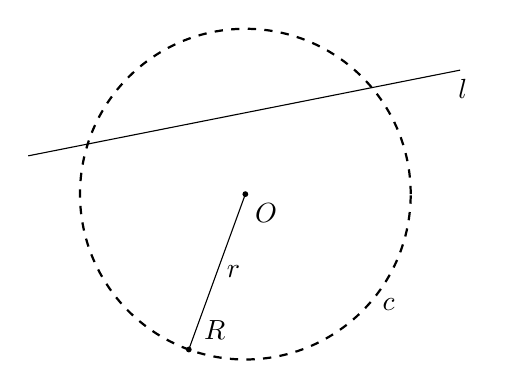
\begin{tikzpicture}[scale=.7]
\coordinate (O) at (0,0);
\node at (2.6,-2) {$c$};
\draw[thick,dashed] (O) circle[radius=3cm];
\fill (O) node[below right] {$O$} circle[radius=1.5pt];
\draw (O) -- node[right] {$r$} ++(-110:3cm) coordinate (R);
\fill (R) circle[radius=1.5pt] node[above right,xshift=2pt] {$R$};
\draw (O) +(170:4cm) -- node[below, near end,xshift=40pt,yshift=8pt] {$l$} ++(30:4.5cm);
\end{tikzpicture}
\vspace*{-8pt}
\selectlanguage{hebrew}
\end{center}
לפי
\L{\ref{s.perpendicular}}
ניתן לבנות אנך ממרכז המעגל
$O$
לקו
$l$.
נסמן ב-%
$M$
את נקודת החיתוך של
$l$
עם האנך. 
$M$
חוצה של המיתר 
$XY$,
כאשר 
$X,Y$
הן נקודות החיתוך של הקו עם המעגל. 
$2s$
הוא אורך המיתר. שימו לב שבתרשים
$s,X,Y$
הם רק הגדרות: טרם בנינו את נקודות החיתוך.
\begin{center}
\selectlanguage{english}
\begin{tikzpicture}[scale=.7]
\coordinate (O) at (0,0);
\node at (2.6,-2) {$c$};
\draw[thick,dashed,name path=circle] (O) circle[radius=3cm];
\fill (O) node[below right] {$O$} circle[radius=1.5pt];
\draw (O) -- node[right] {$r$} ++(-110:3cm) coordinate (R);
\fill (R) node[above right,xshift=2pt] {$R$} circle[radius=1.5pt];
\draw[name path=l] (O) ++(170:4cm) -- node[below, near end,xshift=40pt,yshift=12pt] {$l$} ++(20:8cm);
\path[name intersections={of=circle and l,by={Y,X}}];
\fill (X) node[above left] {$X$} circle[radius=1.5pt];
\fill (Y) node[above right,yshift=2pt] {$Y$} circle[radius=1.5pt];
\draw (O) -- node[below] {$r$} (X);
\path (X) -- ($(X)!.5!(Y)$) coordinate (M);
\fill (M) node[above] {$M$} circle[radius=1.5pt];
\draw (O) -- node[right] {$t$} (M);
\path (X) -- node[above] {$s$} (M);
\path (M) -- node[above] {$s$} (Y);
\draw (O) ++(170:4cm) -- ++(20:3.1cm) -- ++(-70:10pt) -- ++(20:10pt);
\end{tikzpicture}
\vspace*{-6pt}
\selectlanguage{hebrew}
\end{center}
$\triangle OMX$
הוא מעגל ישר זווית, ולכן
$\rule[-5pt]{0pt}{30pt}s^2=r^2-t^2=(r+t)(r-t)$.
$r$
נתון כרדיוס המעגל, ו-%
$t$
הוגדר כאורך של
$OM$,
קטע הקו שבין
$O$
ו-%
$M$.
לפי
\L{\ref{s.direction}}
ניתן לבנות קטעי קו באורך
$t$
מהנקודה 
$O$
בשני הכיוונים
$RO$
ו-%
$OR$.
התוצאה היא שני קטעי קו שאורכם
$r+t,r-t$.

לפי 
\L{\ref{s.root}}
ניתן לבנות קטע קו באורך
$\rule[-5pt]{0pt}{30pt}s=\sqrt{(r+t)(r-t)}$.
שוב לפי
\L{\ref{s.direction}},
ניתן לבנות קטעי קו באורך 
$s$
על הקו הנתון
$l$
מהנקודה
$M$
בשני הכיוונים. הקצה השני של כל אחד מקטעי הקו האלה הוא נקודת חיתוך 
$l$
עם
$c$.

%%%%%%%%%%%%%%%%%%%%%%%%%%%%%%%%%%%%%%%%%%%%%%%%%%%%%%%%%%%%%%%

\section{%
בניית נקודות חיתוך של שני מעגלים%
}\label{s.circle-circle}

\textbf{%
נתון שני מעגלים עם מרכזים
$O_1,O_2$
והדיוסים
$r_1,r_2$.
ניתן לבנות את נקודות החיתוך שלהם
$X,Y$.%
}

עם סרגל ניתן לבנות את קטע הקו
$O_1O_2$
המחבר את שני המרכזים. נסמן את אורכו ב-%
$t$.

\np

\begin{center}
\selectlanguage{english}
\begin{tikzpicture}[scale=1.1]
\coordinate (O1) at (0,0);
\coordinate (O2) at (2.5,0);
\fill (O1) node[below left] {$O_1$} circle[radius=1.5pt];
\fill (O2) node[below right] {$O_2$} circle[radius=1.5pt];
\draw[thick,dashed,name path=circle1] (O1) circle[radius=2cm];
\draw[thick,dashed,name path=circle2] (O2) circle[radius=1.6cm];
\path [name intersections={of=circle1 and circle2,by={X,Y}}];
\draw (O1) -- node[above] {$r_1$} ++(160:2cm);
\draw (O2) -- node[above] {$r_2$} ++(30:1.6cm);
\fill (O1) ++(160:2cm) circle[radius=1.5pt];
\fill (O2) ++(30:1.6cm) circle[radius=1.5pt];
\draw (O1) -- (O2);
\node at (-1.7,1.6) {$c_1$};
\node at (3.8,1.4) {$c_2$};
\draw[<->] (0,-1) -- node[fill=white] {$t$} (2.5,-1);
\node at (6,0) {$t=O_1O_2$};
\end{tikzpicture}
\selectlanguage{hebrew}
\end{center}

\vspace{-1ex}

נסמן ב-%
$A$
את נקודת החיתוך של
$O_1O_2$
עם
$XY$,
ונסמן את האורכים
$q=O_1A,x=XA$.

\vspace{-1ex}

\begin{center}
\selectlanguage{english}
\begin{tikzpicture}[scale=1.1]
\coordinate (O1) at (0,0);
\coordinate (O2) at (2.5,0);
\fill (O1) node[below left] {$O_1$} circle[radius=1.5pt];
\fill (O2) node[below right] {$O_2$} circle[radius=1.5pt];
\draw[thick,dashed,name path=circle1] (O1) circle[radius=2cm];
\draw[thick,dashed,name path=circle2] (O2) circle[radius=1.6cm];
\path [name intersections={of=circle1 and circle2,by={X,Y}}];
\fill (X) node[above,yshift=4pt] {$X$} circle[radius=1.5pt];
\fill (Y) node[below,yshift=-4pt] {$Y$} circle[radius=1.5pt];
\draw[thick,dashed] (O1) -- node[above,xshift=-4pt] {$r_1$} (X);
\draw[thick,dashed] (O2) -- node[above,xshift=4pt] {$r_2$} (X);
\draw[name path=oo] (O1) -- (O2);
\node at (-1.7,1.6) {$c_1$};
\node at (3.8,1.4) {$c_2$};
\draw[name path=xy] (X) -- (Y);
\path[name intersections={of=xy and oo,by={A}}];
\fill (A) node[below left] {$A$} circle[radius=1.5pt];
\path (O1) -- node[below,xshift=-2pt] {$q$} (A);
\path (X) -- node[left,yshift=-2pt] {$x$} (A);
\draw[<->] (0,-1) -- node[fill=white] {$t$} (2.5,-1);
\node at (6,.5) {$t=O_1O_2$};
\node at (6,0) {$q=O_1A$};
\node at (6,-.5) {$x=XA$};
\end{tikzpicture}
\selectlanguage{hebrew}
\end{center}

\vspace{-1ex}

שימו לב שלא בנינו את הנקודה
$A$,
אבל אם נצליח לבנות את האורכים
$q,x$,
לפי 
\L{\ref{s.direction}}
נוכל לבנות את 
$A$
באורך
$q$
מהנקודה
$O_1$
לכיוון
$O_1O_2$.
לפי 
\L{\ref{s.perpendicular}}
ניתן לבנות את האנך ל-%
$O_1O_2$
בנקודה
$A$,
ושוב לפי
\L{\ref{s.direction}}
ניתן לבנות קטעי קו באורך
$x$
מהנקודה
$A$
בשני הכיוונים לאורך האנך. הקצה השני של כל קטע קו
$X,Y$
הוא נקודת חיתוך של שני המעגלים.

\textbf{%
בניית האורך
$q$:}
נסמן
$\rule[-5pt]{0pt}{30pt}d=\sqrt{r_1^2+t^2}$, 
אורך היתר של משולש ישר זווית. ניתן לבנות אותו מ-%
$r_1,t$,
האורכים הידועים של שני הצלעות האחרים: על קו כלשהי נבנה קטע קו
$RS$
באורך
$r_1$,
אחר כך אנך ל-%
$RS$
דרך
$R$,
ולבסוף קטע קו
$RT$
באורך 
$t$
מ-%
$R$
על האנך. אורך היתר
$ST$
שווה ל-%
$d$.
ניתן לבנות את המשולש בכל מקום במישור, לאו דווקא בקירבת המעגלים.

לפי חוק הקוסינוסים ב-%
$\triangle O_1O_2X$:
\erh{12pt}
\begin{equationarray*}{rcl}
r_2^2 &=& t^2 + r_1^2 - 2r_1t\cos\angle XO_1O_2\\
&=& t^2 + r_1^2 - 2tq\\
%2tq &=& (r_1^2+t^2) - r_2^2\\
q&=&\disfrac{(d+r_2)(d-r_2)}{2t}\,.
\end{equationarray*}
לפי
\L{\ref{s.direction}}
ניתן לבנות את האורכים האלה, ולפי
\L{\ref{s.relative-straight}}
ניתן לבנות את
$q$
מהביטויים
$d+r_2,d-r_2,2t$.


\textbf{%
בניית האורך
$x$:}
$\triangle AO_1X$
הוא משולש ישר זווית, ולכן
$\rule[-5pt]{0pt}{30pt}x^2=r_1^2-q^2 =\sqrt{(r_1+q)(r_1-q)}$.
לפי
\L{\ref{s.direction}}
ניתן לבנות
$h =r_1+ q$
ו-%
$k= r_1 - q$,
ולפי
\L{\ref{s.root}}
ניתן לבנות
$\rule[-5pt]{0pt}{20pt}x= \sqrt{hk}$. 

\selectlanguage{english}

